%%%%%%%%%%%%%%%%%%%%%%%%%%%%%%%%%%%%%%%%%
% Programming/Coding Assignment
% LaTeX Template
%
% This template has been downloaded from:
% http://www.latextemplates.com
%
% Original author:
% Ted Pavlic (http://www.tedpavlic.com)
%
% Note:
% The \lipsum[#] commands throughout this template generate dummy text
% to fill the template out. These commands should all be removed when 
% writing assignment content.
%
% This template uses a Perl script as an example snippet of code, most other
% languages are also usable. Configure them in the "CODE INCLUSION 
% CONFIGURATION" section.
%
%%%%%%%%%%%%%%%%%%%%%%%%%%%%%%%%%%%%%%%%%

%----------------------------------------------------------------------------------------
%	PACKAGES AND OTHER DOCUMENT CONFIGURATIONS
%----------------------------------------------------------------------------------------

\documentclass{article}

\usepackage{fancyhdr} % Required for custom headers
\usepackage{lastpage} % Required to determine the last page for the footer
\usepackage{extramarks} % Required for headers and footers
\usepackage[usenames,dvipsnames]{color} % Required for custom colors
\usepackage{graphicx} % Required to insert images
\usepackage{listings} % Required for insertion of code
\usepackage{courier} % Required for the courier font
\usepackage{lipsum} % Used for inserting dummy 'Lorem ipsum' text into the template
\usepackage{amsmath}
\usepackage{booktabs}
\usepackage{bigstrut}
\usepackage{float}
\usepackage{hyperref}
\usepackage{color}
\usepackage{algorithm}
\usepackage{caption}
\usepackage{algpseudocode}

\hypersetup{
    colorlinks   = true,    % Colours links instead of ugly boxes
    urlcolor     = red,    % Colour for external hyperlinks
    linkcolor    = red,    % Colour of internal links
    citecolor    = red      % Colour of citations
}
% Margins
\topmargin=-0.45in
\evensidemargin=0in
\oddsidemargin=0in
\textwidth=6.5in
\textheight=9.0in
\headsep=0.25in

\linespread{1.1} % Line spacing

% Set up the header and footer
\pagestyle{fancy}
\lhead{\hmwkAuthorName} % Top left header
\chead{\hmwkClass\ : \hmwkTitle} % Top center head
\rhead{\firstxmark} % Top right header
\lfoot{\lastxmark} % Bottom left footer
\cfoot{} % Bottom center footer
\rfoot{Page\ \thepage\ of\ \protect\pageref*{LastPage}} % Bottom right footer
\renewcommand\headrulewidth{0.4pt} % Size of the header rule
\renewcommand\footrulewidth{0.4pt} % Size of the footer rule

\setlength\parindent{0pt} % Removes all indentation from paragraphs

%----------------------------------------------------------------------------------------
%	CODE INCLUSION CONFIGURATION
%----------------------------------------------------------------------------------------

\definecolor{MyDarkGreen}{rgb}{0.0,0.4,0.0} % This is the color used for comments
\lstloadlanguages{Perl} % Load Perl syntax for listings, for a list of other languages supported see: ftp://ftp.tex.ac.uk/tex-archive/macros/latex/contrib/listings/listings.pdf
\lstset{language=Perl, % Use Perl in this example
    frame=single, % Single frame around code
    basicstyle=\small\ttfamily, % Use small true type font
    keywordstyle=[1]\color{Blue}\bf, % Perl functions bold and blue
    keywordstyle=[2]\color{Purple}, % Perl function arguments purple
    keywordstyle=[3]\color{Blue}\underbar, % Custom functions underlined and blue
    identifierstyle=, % Nothing special about identifiers                                         
    commentstyle=\usefont{T1}{pcr}{m}{sl}\color{MyDarkGreen}\small, % Comments small dark green courier font
    stringstyle=\color{Purple}, % Strings are purple
    showstringspaces=false, % Don't put marks in string spaces
    tabsize=5, % 5 spaces per tab
    %
    % Put standard Perl functions not included in the default language here
    morekeywords={rand},
    %
    % Put Perl function parameters here
    morekeywords=[2]{on, off, interp},
    %
    % Put user defined functions here
    morekeywords=[3]{test},
    %
    morecomment=[l][\color{Blue}]{...}, % Line continuation (...) like blue comment
    numbers=left, % Line numbers on left
    firstnumber=1, % Line numbers start with line 1
    numberstyle=\tiny\color{Blue}, % Line numbers are blue and small
    stepnumber=5 % Line numbers go in steps of 5
}

% Creates a new command to include a perl script, the first parameter is the filename of the script (without .pl), the second parameter is the caption
\newcommand{\perlscript}[2]{
    \begin{itemize}
        \item[]\lstinputlisting[caption=#2,label=#1]{#1.py}
    \end{itemize}
}
\newcommand{\cppscript}[1]{
    \begin{itemize}
        \item[]\lstinputlisting[]{#1}
    \end{itemize}
}

%----------------------------------------------------------------------------------------
%	DOCUMENT STRUCTURE COMMANDS
%	Skip this unless you know what you're doing
%----------------------------------------------------------------------------------------

% Header and footer for when a page split occurs within a problem environment
\newcommand{\enterProblemHeader}[1]{
    \nobreak\extramarks{#1}{#1 continued on next page\ldots}\nobreak
    \nobreak\extramarks{#1 (continued)}{#1 continued on next page\ldots}\nobreak
}

% Header and footer for when a page split occurs between problem environments
\newcommand{\exitProblemHeader}[1]{
    \nobreak\extramarks{#1 (continued)}{#1 continued on next page\ldots}\nobreak
    \nobreak\extramarks{#1}{}\nobreak
}

%\setcounter{secnumdepth}{0} % Removes default section numbers
\newcounter{homeworkProblemCounter} % Creates a counter to keep track of the number of problems

\newcommand{\homeworkProblemName}{}
\newenvironment{homeworkProblem}[1][Problem \arabic{homeworkProblemCounter}]{ % Makes a new environment called homeworkProblem which takes 1 argument (custom name) but the default is "Problem #"
    \stepcounter{homeworkProblemCounter} % Increase counter for number of problems
    \renewcommand{\homeworkProblemName}{#1} % Assign \homeworkProblemName the name of the problem
    \section{\homeworkProblemName} % Make a section in the document with the custom problem count
    \enterProblemHeader{\homeworkProblemName} % Header and footer within the environment
    }{
    \exitProblemHeader{\homeworkProblemName} % Header and footer after the environment
}

\newcommand{\problemAnswer}[1]{ % Defines the problem answer command with the content as the only argument
\noindent\framebox[\columnwidth][c]{\begin{minipage}{0.98\columnwidth}#1\end{minipage}} % Makes the box around the problem answer and puts the content inside
}

\newcommand{\homeworkSectionName}{}
\newenvironment{homeworkSection}[1]{ % New environment for sections within homework problems, takes 1 argument - the name of the section
    \renewcommand{\homeworkSectionName}{#1} % Assign \homeworkSectionName to the name of the section from the environment argument
    \subsection{\homeworkSectionName} % Make a subsection with the custom name of the subsection
    \enterProblemHeader{\homeworkProblemName\ [\homeworkSectionName]} % Header and footer within the environment
    }{
    \enterProblemHeader{\homeworkProblemName} % Header and footer after the environment
}

%----------------------------------------------------------------------------------------
%	NAME AND CLASS SECTION
%----------------------------------------------------------------------------------------

\newcommand{\hmwkTitle}{homework 03} % Assignment title
\newcommand{\hmwkDueDate}{Tuesday,\ March\ 21,\ 2017} % Due date
\newcommand{\hmwkClass}{Numerical Analysis} % Course/class
\newcommand{\hmwkClassTime}{10:30am} % Class/lecture time
\newcommand{\hmwkClassInstructor}{Jones} % Teacher/lecturer
\newcommand{\hmwkAuthorName}{102061149 Fu-En Wang} % Your name

%----------------------------------------------------------------------------------------
%	TITLE PAGE
%----------------------------------------------------------------------------------------

\title{
    \vspace{2in}
    \textmd{\textbf{\hmwkClass:\ \hmwkTitle}}\\
    \normalsize\vspace{0.1in}\small{Due\ on\ \hmwkDueDate}\\
    \vspace{3in}
}

\author{\textbf{\hmwkAuthorName}}
\date{} % Insert date here if you want it to appear below your name

%----------------------------------------------------------------------------------------

\begin{document}

\maketitle
\newpage


\section{Introduction}
For modern circult design, the scale of circult is always such large that human cannot handle it manually. To overcome this, 
we frequently use a lot of EDA tool such as \textbf{hspice} to solve these problems. However, the license of these EDA tool is 
usualy expensive. As a result, EDA provider such as \textbf{Synopsys} benefits a lot from it every year, which means these
circult analysis technology is quite valuable. \newline
In this project, we will implement several simple \textbf{Resistor Networks} and use \textbf{LU Decomposition} to analyze it.
\subsection{Resistor Networks}
Each resistor networks only consists of several resistors as shown in Figure \ref{fig:resistor_network}.
\begin{figure}[H]
    \centering
    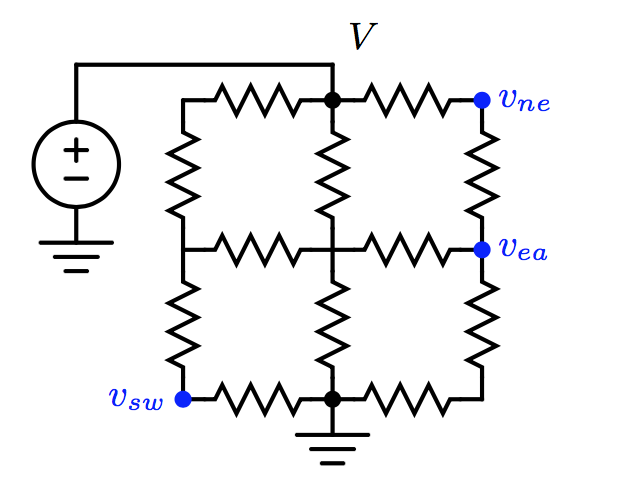
\includegraphics[width=0.5\textwidth]{src/resistor_network.png}
    \caption{Simple resistor network}
    \label{fig:resistor_network}
\end{figure}
In this assignment, there are six networks to implement:
\begin{enumerate}
    \item 2 resistors each side and resistance is $1K\Omega$
    \item 4 resistors each side and resistance is $500\Omega$
    \item 10 resistors each side and resistance is $200\Omega$
    \item 20 resistors each side and resistance is $100\Omega$
    \item 40 resistors each side and resistance is $50\Omega$
    \item 50 resistors each side and resistance is $40\Omega$
\end{enumerate}
For each of them, we have to show the equivalent resistance and the voltage of $V_{ne}$, $V_{ea}$ and $V_{sw}$.
\newpage

\section{Implementation}
\subsection{Algorithm}
To model the problem into $A$ and $b$, I divide the network into two segments by horizontal and vertical resistor as shown in
Figure \ref{fig:resistor_network}. And then update matrix A and b with \textbf{Algorithm 1.4.1} in class material.
\begin{algorithm}[htb]
    \caption*{\textbf{Algorithm 1.4.1} System Equation for a Resistor Network}
    \label{algo:resistor_network}
    \begin{algorithmic}
        \State For a network with N nodes in each side, create $N^2 \times N^2$ zero matrix A and $N^2$ zero vector b.
        \State nodeIndex = 0
        \State G = $resistance^{-1}$
        \For{each i $\in$ \{1 ... N\}}
            \For{ each j $\in$ \{1 ... N-1\}}
                \State A[nodeIndex][nodeIndex] += G
                \State A[nodeIndex][nodeIndex+1] -= G
                \State A[nodeIndex+1][nodeIndex+1] += G
                \State A[nodeIndex+1][nodeIndex] -= G
                \State nodeIndex += 1
            \EndFor
            \State nodeIndex += 1
        \EndFor
        \State nodeIndex = 0
        \For{each i $\in$ \{1 ... N-1\}}
            \For{each j $\in$ \{1 ... N\}}
                \State A[nodeIndex][nodeIndex] += G
                \State A[nodeIndex][nodeIndex+N] -= G
                \State A[nodeIndex+N][nodeIndex+N] += G
                \State A[nodeIndex+N][nodeIndex] -= G
                \State nodeIndex += 1
            \EndFor
        \EndFor
        \For{v,i $\in$ voltage and index at fixed voltage point}
            \State A[i] = 0
            \State A[i][i] = 1
            \State b[i] = v
        \EndFor
        \State LU = luDecompose(A)
        \State Y = forwardSub(LU, b)
        \State X = backwardSub(LU, Y)
        \State X is the voltage of each node.
    \end{algorithmic}
\end{algorithm}


\section{Discussion}
\subsection{Complexity}
\label{sec:complexity}
In all the folowing part, I will refer $N$ as the square of the number of nodes at each side of networks. For the network in 
Figure \ref{fig:resistor_network}, N is $3 \times 3 = 9$. \newline
When solving the problem, the most time-comsuming part is the \textbf{LU Decomposition}, which is $O(n^3)$. As a result, the
system is a {\boldmath$O(n^3)$} problem.

\subsection{Performance Evaluation}
In this project, I use five numbers to indicate the efficiency of our method:
\begin{enumerate}
    \item \textbf{Runtime}(total execution time of program)
    \item \textbf{PROBLEM}(execution time of modeling problem into martrix A and vector b)
    \item \textbf{LU}(time taken by LU Decomposition)
    \item \textbf{FWD}(time taken by forward substitution)
    \item \textbf{BCK}(time taker by backward substitution)
\end{enumerate}
The detail result of each resistor networks is show in Table \ref{tab:result}
\begin{table}[htbp]
  \centering
    \begin{tabular}{|c|c|c|c|c|c|c|}
    \hline
    \textbf{N}   & \textbf{9}   & \textbf{25}  & \textbf{121} & \textbf{441} & \textbf{1681} & \textbf{2601} \bigstrut\\
    \hline
    R(each) & 1000 & 500 & 200 & 100 & 50  & 40 \bigstrut\\
    \hline
    R(equivalent) & 1000 & 681.818182 & 376.009408 & 229.423008 & 136.042809 & 114.395519 \bigstrut\\
    \hline
    $V_{ne}$ & 0.75 & 0.7 & 0.648693 & 0.622178 & 0.603088 & 0.598084 \bigstrut\\
    \hline
    $V_{ea}$ & 0.5 & 0.5 & 0.5 & 0.5 & 0.5 & 0.5 \bigstrut\\
    \hline
    $V_{sw}$ & 0.25 & 0.3 & 0.351307 & 0.377822 & 0.396912 & 0.401916 \bigstrut\\
    \hline
    Runtime(s) & 0.003 & 0.003 & 0.007 & 0.2 & 9.948 & 36.1 \bigstrut\\
    \hline
    PROBLEM(s) & 1.50E-05 & 2.10E-05 & 0.000199 & 0.001173 & 0.020578 & 0.052503 \bigstrut\\
    \hline
    LU(s) & 2.00E-06 & 3.30E-05 & 0.003537 & 0.194482 & 9.89144 & 35.9966 \bigstrut\\
    \hline
    FWD(s) & 1.00E-06 & 5.00E-06 & 4.40E-05 & 0.000489 & 0.008348 & 0.017034 \bigstrut\\
    \hline
    BCK(s) & 1.00E-06 & 3.00E-06 & 4.60E-05 & 0.000532 & 0.010656 & 0.019895 \bigstrut\\
    \hline
    \end{tabular}%
  \caption{Experiment result}
  \label{tab:result}%
\end{table}%

\subsection{Runtime and LU}
Because LU Decomposition should be the most time-consuming part of algorithm, so after N is large enough, LU should be very close to
Runtime. Figure \ref{fig:runtime_lu} shows the result of Runtime/LU and $N^3$ with log-scale:
\begin{figure}[H]
    \centering
    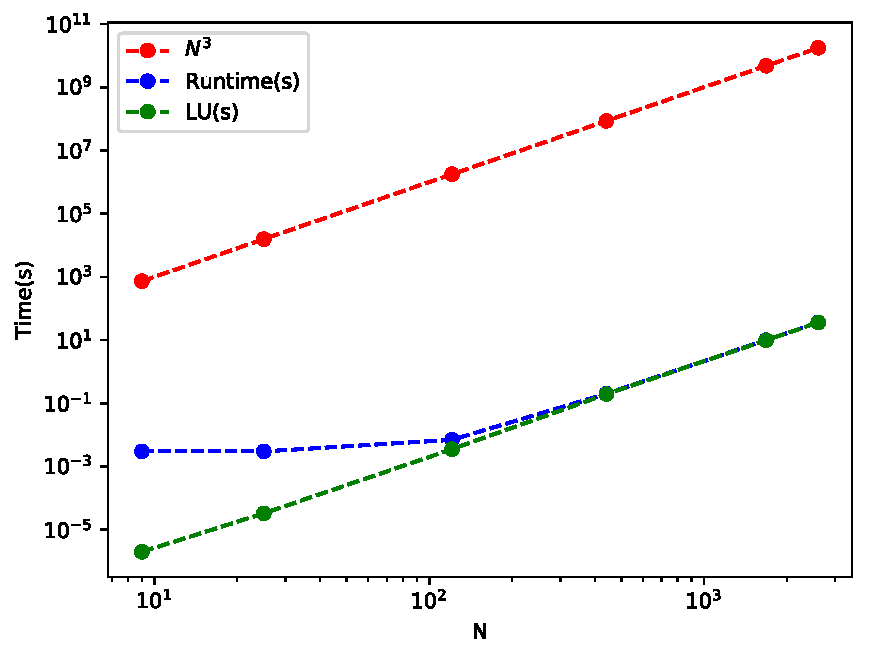
\includegraphics[width=0.65\textwidth]{src/runtime_lu.pdf}
    \caption{Runtime/LU vs N}
    \label{fig:runtime_lu}
\end{figure}
Because when N is small, execution time will have huge error, so we should ignore former part of the line of Runtime. However, when
N is large, we can see that Runtime and LU almost overlap and their slope is same as $N^3$, which means the system is a 
{\boldmath$O(n^3)$} problem and satisfies my analysis in Section \ref{sec:complexity}.

\subsection{Forward/Backward Substitution}
Because the complixity of Forward/Backward Substitution is {\boldmath$O(n^2)$} as we discuss in last homework assignment, the
slope of them should be same as $N^2$ in log-scale plot. Figure \ref{fig:fwd_bck} shows the result with log-scale.
\begin{figure}[H]
    \centering
    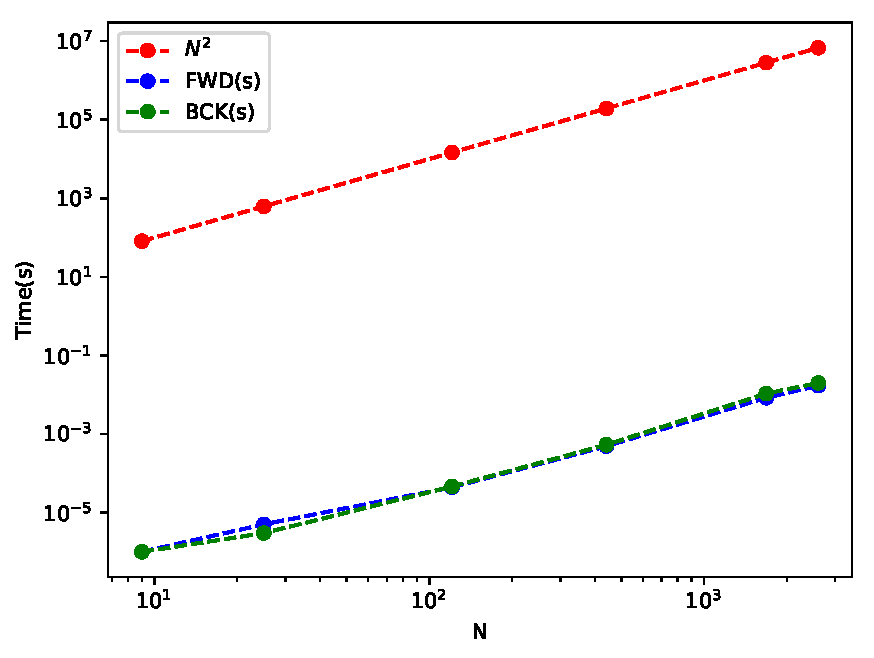
\includegraphics[width=0.65\textwidth]{src/fwd_bck.pdf}
    \caption{FWD/BCK vs N}
    \label{fig:fwd_bck}
\end{figure}
From Figure \ref{fig:fwd_bck}, we can clearly see that the slope of FWD and BCK is same as $N^2$, which means they are
{\boldmath$O(n^2)$} problem.

\section{Code Usage}
To compile the code, just type \textbf{\$ g++ hw03.cpp MAT.cpp VEC.cpp} in terminal. \newline
To run the program, use \textbf{\$ ./a.out 10}, 10 means there are 10 resistors at each side of the resistor network.


\end{document}








